% !TeX root = ../../../book.tex

\subsection{更多示例}

在掌握这两个定理后,让我们通过若干关系示例来加深理解。对于每个例子,判断其是否为等价关系:如果是,则描述其等价类;如果不是,则根据定理说明不是的原因。

\begin{example}
    先从一个简单的例子开始。\\
    回顾示例 \ref{ex:example6.2.9} 定义的相等关系。我们已经解释过,``$=$''在任意集合上都是等价关系,其等价类即各元素自身构成的单元素集。例如,在集合 $\mathbb{N}$ 中,$[1]_{=} = \{1\}, [2]_{=} = \{2\}$,依此类推。所有等价类都是\emph{单元素集}(集合中只有一个元素)。
\end{example}

\begin{example}
    再来看一个相对简单的例子。\\
    回顾示例 \ref{ex:example6.2.5} 中定义的整数集 $\mathbb{Z}$ 上的奇偶关系。这是一个等价关系,让我们来证明这一点。

    \begin{proof}
        设 $a, b, c \in \mathbb{Z}$ 为任意整数。
        \begin{itemize}
            \item \textbf{自反性}:不难发现 $(a,a) \in R$,因为 $a$ 与其自身有相同的奇偶性。因此 $R$ 具有自反性。
            \item \textbf{对称性}:假设 $(a,b) \in R$,则 $a$ 和 $b$ 具有相同的奇偶性。显然,$b$ 和 $a$ 也具有相同的奇偶性,故 $(b,a) \in R$。因此 $R$ 具有对称性。
            \item \textbf{传递性}:假设 $(a,b) \in R$ 且 $(b,c) \in R$。
            \begin{itemize}
                \item 若 $a$ 是奇数,则 $b$ 和 $c$ 也都是奇数。
                \item 若 $a$ 是偶数,则 $b$ 和 $c$ 也都是偶数。
            \end{itemize}
            无论哪种情况,$a$ 和 $c$ 都具有相同的奇偶性,故 $(a,c) \in R$。因此 $R$ 具有传递性。
        \end{itemize}
        综上,由于 $R$ 具有自反性、对称性和传递性,所以 $R$ 是一个等价关系。
    \end{proof}

    这意味着等价类集合 $\mathbb{Z}/R$ 构成 $\mathbb{Z}$ 的划分。让我们来确定该划分。

    考虑 $[0]_R$,它表示所有与 $0$ 奇偶性相同的整数集合,即全体\emph{偶数}。因此,在此情况下,
    \[\mathbb{Z}/R = \{O_{\mathbb{Z}}, E_{\mathbb{Z}}\}\]
    其中 $O_{\mathbb{Z}}$ 为奇数集,$E_{\mathbb{Z}}$ 为偶数集。这两个等价类都是无穷大的。
\end{example}

\begin{example}
    回顾示例 \ref{ex:example6.2.6} 中定义的 $\mathbb{R}$ 上的顺序关系。该关系是等价关系吗?我们可以通过逐一检验其性质来判断。注意到对于任意 $x \in \mathbb{R}$,均有 $(x, x) \notin R$(因为 $x \nless x$)。因此 $R$ 缺乏自反性,故它不是等价关系。(此外,$R$ 虽具有传递性,但缺乏对称性。)

    为何严格顺序关系不能成为等价关系?自反性对等价关系为何重要?考虑\emph{等价类}的概念:等价关系应将整个集合划分为若干子集,使每个元素都能通过所属子集被标识。若关系不具自反性,则某些元素将不属于其自身的``等价类'',这显然不符合要求!

    (进一步思考:自反的顺序关系 $\le$ 是否为等价关系?请说明理由。)
    
    换言之,$\mathbb{R}$ 上的``$<$''关系无法将实数集划分。结合定理 \ref{theorem6.4.10} 的\emph{逆否命题},可推知 ``$<$''\emph{不是}等价关系。
\end{example}

\begin{example}
    定义 $\mathbb{R} \times \mathbb{R}$ 上的关系 $\sim$ 为
    \[(x, y) \sim (u, v) \iff x \le u \land y \le v\]
    即使不逐条检验性质,我们也可以推断出它是否是等价关系。为此,我们选取集合中的一个特定元素,并查看与该特定元素相关的所有元素。在下图中,我们使用 $(1, 1)$ 作为这个特定元素。

    \begin{center}
        {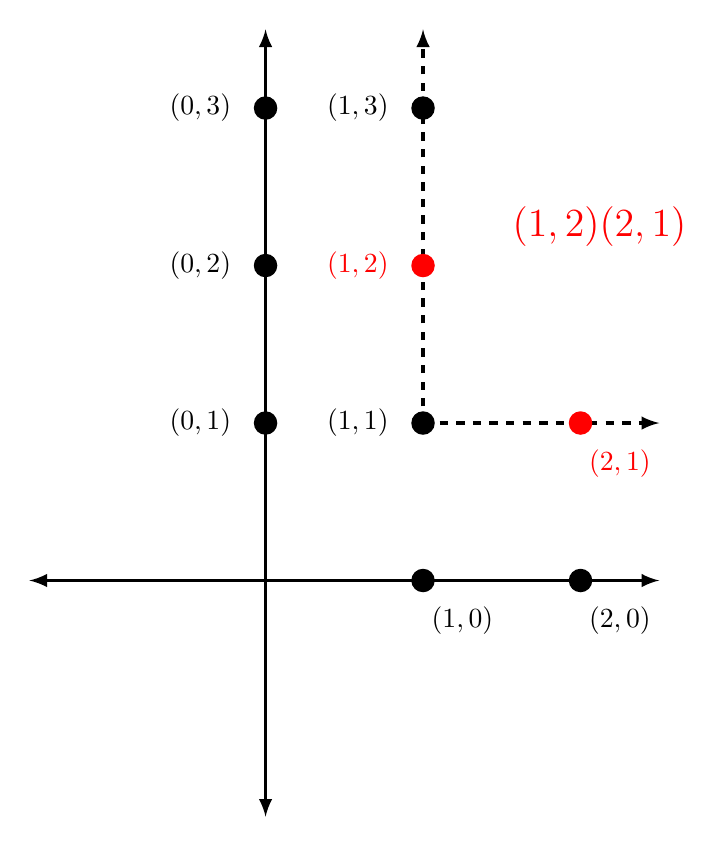
\begin{tikzpicture}[very thick,scale=2]
            \draw[latex-latex] (-1.5,0) -- (2.5,0); 
            \draw[latex-latex] (0,-1.5) -- (0,3.5); 
            \foreach \x in  {1,2}
            {
                \node at (\x, 0)[circle,fill,inner sep=3pt]{};
                \draw[shift={(\x+0.25,-0.1)}] node[below] {$(\x, 0)$};
                
            }
            \foreach \y in  {1,2,3}
            {
                \node at (0, \y)[circle,fill,inner sep=3pt]{};
                \draw[shift={(-0.15, \y)}] node[left] {$(0, \y)$};
            }
    
            \draw[dashed,-latex] (1,1) -- (2.5,1); 
            \draw[dashed,-latex] (1,1) -- (1,3.5); 
            \foreach \y in  {1,3}
            {
                \node at (1, \y)[circle,fill,inner sep=3pt]{};
                \draw[shift={(0.85, \y)}] node[left] {$(1, \y)$};
            }
    
            \node[red] at (1, 2)[circle,fill,inner sep=3pt]{};
            \draw[color=red, shift={(0.85, 2)}] node[left] {$(1, 2)$};
            \node[red] at (2, 1)[circle,fill,inner sep=3pt]{};
            \draw[color=red, shift={(2.25, 0.9)}] node[below] {$(2, 1)$};
    
            \draw[color=red, font=\Large, shift={(1.5, 2.25)}] node[right] {$(1,2) \nsim (2,1)$};
        \end{tikzpicture}}
    \end{center}

    请注意,$\sim$ 要求一个点必须位于另一点的``右上方''方可关联。同时,由于不等式是``$\le$'',因此第二个点不必\emph{严格}位于上方或右侧。

    我们可以从上图看到,$(1, 2) \sim (1, 1)$(因为 $1 \le 1$ 且 $1 \le 2$),同理 $(1, 1) \sim (2, 1)$。故 $(1, 2)$ 与 $(2, 1)$ 均与 $(1, 1)$ 关联。若 $\sim$ 是\emph{等价关系},则 $(2, 1)$ 与 $(1, 2)$ 必须彼此关联(因为同属 $(1, 1)$ 的等价类)。然而遗憾的是,$(1, 2) \nsim (2, 1)$,因为后者位于前者的``左下方'',不满足 $\sim$ 的定义。

    这意味着所有与 $(1, 1)$ 关联的元素\textbf{无法}构成``封闭集合'',从数学上讲,这些元素的集合不是一个等价类。因此,$\sim$ \textbf{不是}一个等价关系。

    请进一步分析 $\sim$ 的性质:是否具有自反性?是否具有对称性?是否具有传递性?请说明理由。此过程将再次验证 $\sim$ 不是一个等价关系。建议遇到新定义的关系时采用类似的分析:若能明确其``等价类'',则有助于理解等价关系的构造;若不能,则可积累反例构造的经验。
\end{example}

\subsubsection*{[选学] $\mathbb{Z}$ 是如何从 $\mathbb{N} \times \mathbb{N}$ 上的等价关系生成的}

回忆第 \ref{ch:chapter03} 章的习题:要求证明自然数对的特定性质,并声称此过程构建了整数集。重审视习题 \ref{exc:exercises3.11.22},其最后三部分要求证集合 $P = \mathbb{N} \times \mathbb{N}$ 上的关系 $R$ 是等价关系(已证其自反性、对称性及传递性)。

还记得第 \ref{ch:chapter03} 章中的那道复杂习题吗?它要求证明自然数对的性质,并声称此过程证明了整数的存在性。重新审视习题 \ref{exc:exercises3.11.22},你会发现问题的最后三部分要求证明集合 $R$ 是集合 $P = \mathbb{N} \times \mathbb{N}$ 上的\textbf{等价关系}。仔细阅读一下!你已经证明了 $R$ 具有自反性、对称性和传递性。

该练习表明(此处略去细节)任何负整数都可以表示为两个整数之差为该负整数的\textbf{等价类}。也就是说
\[-1 \;\text{``$=$''}\; [(1, 2)]_R = \{(1, 2),(2, 3),(3, 4), \dots \}\]
同理
\[-3 \;\text{``$=$''}\; [(1, 4)]_R = \{(1, 4),(2, 5),(3, 6), \dots \}\]
以上只是一个直观的解释,从数学上讲并不严格,但核心思想就在于此!
